\documentclass[tikz]{standalone}
\usepackage{pgfplots}
\pgfplotsset{compat=1.15}
\usepackage{mathrsfs}
\usetikzlibrary{arrows,calc}
\usepackage{tkz-euclide}
\pagestyle{empty}

\definecolor{AngleClr}{rgb}{0,0.39215686274509803,0}
\definecolor{ShapeClr}{rgb}{0.6,0.2,0}
\definecolor{BlueSqr}{RGB}{5,81,163}
\definecolor{RedSqr}{RGB}{199, 28, 16}
\definecolor{YellowClr}{RGB}{191, 159, 0}

\begin{document}

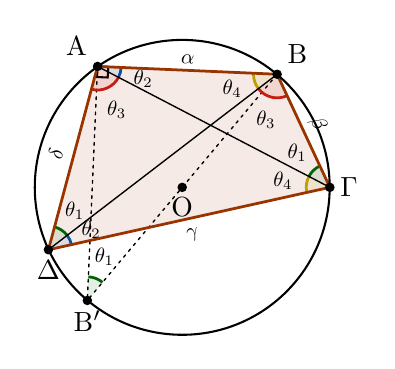
\begin{tikzpicture}[scale=.75]
\tkzSetUpLine[line width=1pt,color=black]
\tkzSetUpPoint[fill=black]


\tkzDefPoint(50:2.5){B}
\tkzDefPoint(125:2.5){A}
\tkzDefPoint(205:2.5){D}
\tkzDefPoint(0:2.5){C}


\tkzDefTriangleCenter[circum](A,B,C) \tkzGetPoint{O}
\tkzDefPointBy[symmetry=center O](B) \tkzGetPoint{B'}

\tkzFillPolygon[fill=ShapeClr,fill opacity=0.1](A,B,C,D)

\tkzDrawSegments[line width=0.5pt,color=black,dashed,dash pattern=on 1pt off 1.75pt](A,B' B,B')

\tkzMarkRightAngle[line width=0.75pt, size=.18,color=black](B,A,B')

\tkzFillAngle[fill=AngleClr,size=.4,fill opacity=0.1](B,B',A)
\tkzMarkAngle[line width=1pt,color=AngleClr,size=.4](B,B',A)
\tkzLabelAngle[pos=0.8](B,B',A){\scalebox{0.75}{$\theta_1$}}

\tkzFillAngle[fill=AngleClr,size=.4,fill opacity=0.1](B,D,A)
\tkzMarkAngle[line width=1pt,color=AngleClr,size=.4](B,D,A)
\tkzLabelAngle[pos=0.8](B,D,A){\scalebox{0.75}{$\theta_1$}}

\tkzFillAngle[fill=AngleClr,size=.4,fill opacity=0.1](B,C,A)
\tkzMarkAngle[line width=1pt,color=AngleClr,size=.4](B,C,A)
\tkzLabelAngle[pos=0.8](B,C,A){\scalebox{0.75}{$\theta_1$}}


\tkzFillAngle[fill=BlueSqr,size=.4,fill opacity=0.1](C,D,B)
\tkzMarkAngle[line width=1pt,color=BlueSqr,size=.4](C,D,B)
\tkzLabelAngle[pos=0.8](C,D,B){\scalebox{0.75}{$\theta_2$}}

\tkzFillAngle[fill=BlueSqr,size=.4,fill opacity=0.1](C,A,B)
\tkzMarkAngle[line width=1pt,color=BlueSqr,size=.4](C,A,B)
\tkzLabelAngle[pos=0.8](C,A,B){\scalebox{0.75}{$\theta_2$}}


\tkzFillAngle[fill=RedSqr,size=.4,fill opacity=0.1](D,A,C)
\tkzMarkAngle[line width=1pt,color=RedSqr,size=.4](D,A,C)
\tkzLabelAngle[pos=0.8](D,A,C){\scalebox{0.75}{$\theta_3$}}

\tkzFillAngle[fill=RedSqr,size=.4,fill opacity=0.1](D,B,C)
\tkzMarkAngle[line width=1pt,color=RedSqr,size=.4](D,B,C)
\tkzLabelAngle[pos=0.8](D,B,C){\scalebox{0.75}{$\theta_3$}}


\tkzFillAngle[fill=YellowClr,size=.4,fill opacity=0.1](A,C,D)
\tkzMarkAngle[line width=1pt,color=YellowClr,size=.4](A,C,D)
\tkzLabelAngle[pos=0.8](A,C,D){\scalebox{0.75}{$\theta_4$}}

\tkzFillAngle[fill=YellowClr,size=.4,fill opacity=0.1](A,B,D)
\tkzMarkAngle[line width=1pt,color=YellowClr,size=.4](A,B,D)
\tkzLabelAngle[pos=0.8](A,B,D){\scalebox{0.75}{$\theta_4$}}


\tkzDrawSegments[line width=0.5pt,color=black](A,C B,D)

\tkzDrawPolygon[color=ShapeClr](A,B,C,D)

\tkzDrawCircle[line width=0.75pt,color=black](O,A)


\tkzDrawPoints[size=3](A,B,C,D,B',O)

\tkzLabelPoint[above left](A){$\rm A$}
\tkzLabelPoint[above right](B){$\rm B$}
\tkzLabelPoint[right](C){$\rm \Gamma$}
\tkzLabelPoint[below](D){$\rm \Delta$}
\tkzLabelPoint[below](O){$\rm O$}
\tkzLabelPoint[below](B'){$\rm B'$}

\tkzLabelSegments[above=-0.05cm,sloped](A,B){\scalebox{0.75}{$\alpha$}}
\tkzLabelSegments[above=-0.05cm,sloped](B,C){\scalebox{0.75}{$\beta$}}
\tkzLabelSegments[below,sloped](C,D){\scalebox{0.75}{$\gamma$}}
\tkzLabelSegments[above,sloped](D,A){\scalebox{0.75}{$\delta$}}

\end{tikzpicture}

\end{document}
